Polynomials provide a natural way to construct new rings out of old ones.
Rings of polynomials inherit some nice structure from their coefficient rings, particularly if those rings are domains.
\begin{center}
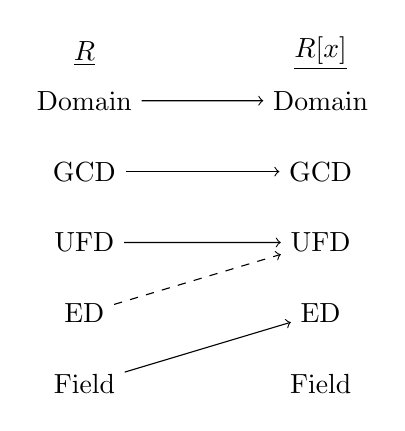
\begin{tikzpicture}[scale=0.3]
  \node (fld1) at (-5,0)  {Field};
  \node (fld2) at ( 5,0)  {Field};
  \node (ed1)  at (-5,3)  {ED};
  \node (ed2)  at ( 5,3)  {ED};
  \node (ufd1) at (-5,6)  {UFD};
  \node (ufd2) at ( 5,6)  {UFD};
  \node (gcd1) at (-5,9)  {GCD};
  \node (gcd2) at ( 5,9)  {GCD};
  \node (dom1) at (-5,12) {Domain};
  \node (dom2) at ( 5,12) {Domain};
  \node (lab1) at (-5,14) {\(\underline{R}\)};
  \node (lab2) at ( 5,14) {\(\underline{R[x]}\)};

  \draw [->] (fld1) edge (ed2);
  \draw [->, dashed] (ed1)  edge (ufd2);
  \draw [->] (ufd1) edge (ufd2);
  \draw [->] (gcd1) edge (gcd2);
  \draw [->] (dom1) edge (dom2);
\end{tikzpicture}
\end{center}
One might expect that detecting irreducibles and finding irreducible factorizations would be more difficult in \(\ZZ[x]\), say, than in \(\ZZ\), but in fact the opposite is true.
This is ultimately due to the existence of the derivative on \(R[x]\) and to some other aspects of the structure of \(R[x]\) which will be explored later.

(@@@) We've seen here that if \(R\) is a UFD, then \(R[x]\) is also a UFD, but have not seen any kind of algorithm which computes factorizations in \(R[x]\).
In the exercises of this and the next section we construct algorithms which work in some important special cases, including \(\ZZ\) and \(\ZZ/(p)\).
